


\section{The North Atlantic Oscillation}

    % The North Atlantic Oscillation (NAO) is a recurrent variation in air pressure between the Arctic and the subtropical Atlantic. It is characterised by low pressure system situated over Iceland and a high pressure system over the Azores islands, west of Portugal. In the Northern Hemisphere air rotates counterclockwise around points of low pressure, and clockwise around points of high pressure. This means that as the NAO becomes more pronounced, meaning a larger and clearer air pressure difference between the two points, a conveyor belt can form which accelerates air parcels towards the middle latitudes of the western parts of Europe. The signifficance of this phenomenon is large as it can affect climate, i.e. a pronounced NAO leads to a warmer and wetter winter in Northern Europe, while the oppositive leads to colder and drier winter weather. Agriculture, water management, energy production, fishery health and population, bird migration and other things are all affected by the state of the NAO \citep{Hurrell2003}. As these changes in climate occure simaltaniusly to the change in air pressure far away, the NAO and is a telaconnection. Amoungst a dozen telaconnections in the northerm hemisphere, the NAO is one of the most prominant alongside the El Ni\~no Southern Oscillation (ENSO). 
    
    % On a temporal scale, the NAO fluctuates daily; where the magnitude of the change can be both large and small, with seemingly no apparent pattern. For a long time no signifficant ability to predict future NAO behaviour was displayed. At the start of the 21st century \cite{AtmosphericGCMResponsetoExtratropicalSSTAnomaliesSynthesisandEvaluation} and \cite{hoerling2001} report a small predictability due to a connection between extratropical sea surface temperature anomalies and the NAO, while \cite{Thompsondoi:https://doi.org/10.1029/134GM05} reports coupling of the NAO to stratospheric processes during winter.
    % The most recent advancements in the field, such as those by \cite{Athanasiadis2020}, \cite{Dunstone2016}, \cite{Scaifehttps://doi.org/10.1002/2014GL059637} and \cite{Smith2020}, demonstrate the skilful ability to predict the NAO to near decadal timescales through climate models \citep{Klavans2021}. The most notable of which is \cite{Smith2020}, where it is argued that decadal predictability of the NAO emerges in large multi-model ensembles. The above are in agreement that, in an unknown ratio, the accuracy of the model is tied to the initialisation of the state of the ocean and to external atmospheric forcings.

    % To quantify the change in the NAO the concept of an NAO Index is introduced. The index is calculated based on the magnitude of air pressure anomaly compared to a standard deviation obtained from a long-term record. When the anomaly observed is that of lower air pressure than standard over Iceland and higher air pressure over the Azores, and thus a greater gap in air pressure between the two points, the NAO Index is defined to be positive. The greater the pressure difference, the higher the index value. The opposite condtions, with higher than standard air pressure over Iceland and lower than standard over the Azores, are defined as a negative NAO Index phase. 


    
    The North Atlantic Oscillation (NAO) is a recurring air pressure fluctuation between the Arctic and the subtropical Atlantic. It is marked by a low-pressure system over Iceland and a high-pressure system over the Azores islands situated west of Portugal. In the Northern Hemisphere, air circulates anti-clockwise around areas of low pressure and clockwise around high pressure. When the NAO intensifies, meaning the air pressure difference between these two points grows, it forms a 'conveyor belt' that speeds up air masses towards the mid-latitudes of western Europe. This has wide-ranging implications, affecting everything from climate and agriculture to energy production and even bird migration \citep{Hurrell2003}. A strong NAO usually brings a warmer, wetter winter in Northern Europe, while the opposite results in colder, drier conditions. Because these climatic changes occur in sync with distant air pressure variations, the NAO is a type of teleconnection. Among various teleconnections in the Northern Hemisphere, the NAO is particularly prominent, along with the El Niño Southern Oscillation (ENSO).

    On a temporal scale, the NAO fluctuates daily; where the magnitude of the change can be both large and small, with seemingly no apparent pattern. For a long time, no significant ability to predict future NAO behaviour was displayed. At the beginning of the 21st century, \cite{AtmosphericGCMResponsetoExtratropicalSSTAnomaliesSynthesisandEvaluation} and \cite{hoerling2001} report a small predictability due to a connection between extratropical sea surface temperature anomalies and the NAO, while \cite{Thompsondoi:https://doi.org/10.1029/134GM05} reports a coupling of the NAO with stratospheric processes during winter.
    The most recent advances in the field, such as those of \cite{Athanasiadis2020}, \cite{Dunstone2016}, \cite{Scaifehttps://doi.org/10.1002/2014GL059637} and \cite{Smith2020}, demonstrate the skilful ability to predict the NAO on near decadal timescales through climate models \citep{Klavans2021}. The most notable of which is \cite{Smith2020}, where it is argued that the decadal predictability of the NAO emerges in large multi-model ensembles. The above are in agreement that, in an unknown ratio, the accuracy of the model is tied to the initialisation of the state of the ocean and to external atmospheric forcings.
    
    To gauge the NAO's fluctuations, an NAO Index is used. This index measures air pressure anomalies against a long-term standard deviation. When there is lower-than-average pressure over Iceland and higher-than-average over the Azores, resulting in a larger pressure gap, the NAO Index is deemed positive. The opposite conditions produce a negative NAO Index.
    
    

\section{European Windstorms and the NAO}
    In 650 BCE researchers from the Babylonian Institute for Seasonal Forecasts proposed a novel at the time method for producing month-long climate trends based on constellations appearing in the night sky \citep{Ossendrijver+2021+223+258}. 
    
    In 1992 the European Centre for Medium-Range Weather Forecasts (ECMWF) was among the first to implement ensemble forecasting. Ensemble forecasting is a method of computational forecasting where the evolution of an environmental system is simulated based on physical laws and boundary conditions from a starting point. Because of the size and complexity of individual components, it is not possible to have a set the initial state of the system with absolute certainty, nor to simulate the behaviour of constituents on the micro level. Because of this inherent uncertainty, individual runs of a simulation, called members, are likely to divert by a small degree from each other in the early stages of a simulation. Similarly to the illustrative metaphor by an unknown meteorologist:
    
    \begin{displayquote}
        \textit{one flap of a seagull's wings would be enough to alter the course of the weather forever...}
    \end{displayquote}
    
    , later replaced with a butterfly by Lorenz \citep{Lorenz1963}, so do the ensemble members go on to simulate different 'worlds'. The simulations themselves remain physically possible, but they can differ significantly from each other. Nevertheless, by creating a probabilistic prognosis based on the frequency of meteorological phenomena appearing in each member, atmospheric scientists have been able to successfully predict surface variables such as temperature or precipitation with increasing accuracy. The ability to skilfully predict windstorms caused by extratropical cyclones is not explored as well \citep{Degenhardt2023}. In the next section, we will review recent advances and current limitations in windstorm forecasting.



    \subsection{A brief history of windstorm forecasting}
        The primary goal of windstorm prediction is to produce accurate and reliable forecasts for the public and private sectors. As such a focus is placed on the statistical relationship between windstorms and indices such as the NAO, which affect the climate. Although much has been achieved in terms of understanding the workings of the NAO and extratropical storms, there is no established relationship that links a particular state of the NAO with a confident forecast of the frequency and intensity of the windstorms. Forecasts are produced through ensemble modells in local or global climate simulations. 
        
        In an experiment using the National Centre for Atmospheric Research (NCAR) general circulation model, \cite{TheEffectsofNorthAtlanticSSTandSeaIceAnomaliesontheWinterCirculationinCCM3PartIMainFeaturesandStormTrackCharacteristicsoftheResponse} discusses the tendency of storm tracks to follow a meridonal flow during positive NAO states and a zonal flow during negative NAO states. \cite{Hurrell2003} make simmilar conclusions and, in addition, based on observations from 1958 to 2001 of mean wind speed (1000~hPa, 200~hPa) and mean sea level pressure, shows that meridonal winds are stronger and more characteristic of boreal winter (December - February), while zonal winds tend to be weaker and more characteristic of boreal summer (June - August). \citeauthor{Hurrell2003} ilustrate this in Figure \ref{fig:vectorwinds}. We validate these results using research tools from \cite{ClimateReanalyzer2023} and establish their persistence over a shifted time frame of 1980 to 2019, as illustrated in Figures \ref{fig:CR23_DJF_1000hPa_wind} and \ref{fig:CR23_JJA_1000hPa_wind}.
    
        \begin{figure}
            \centering
            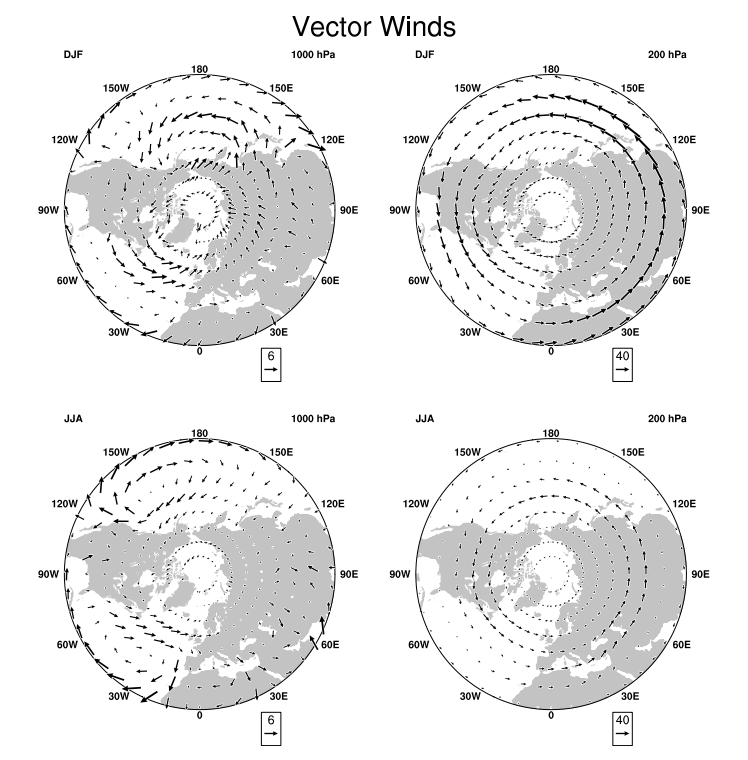
\includegraphics[width=\textwidth]{figures/vectorwinds.png}
            \caption{Figure and caption sourced from \cite{Hurrell2003}. Mean vector winds for (top) boreal winter (December-February) and (bottom) boreal summer (June-August) for (left) 1000~hPa and (right) 200~hPa over 1958-2001. The scaling vectors are indicated in the boxes and are given in units of m/s.}
            \label{fig:vectorwinds}
        \end{figure}
    
        \cite{ClimateReanalyzer2023} provides access to common environmental variables through reanalysis data from the ECMWF and NCEP, as well as indices and gridded observations from NOAA. In addition, they offer access to tools for the creation of custom plots. In addition to the appendix figures that confirm 1000hPa wind vectors, we include Figures \ref{fig:CR_10m_wind_DJF} and \ref{fig:CR_10m_wind_JJA}. These depict average 10m wind speed during boreal winter (DJF) and summer (JJA) from 1950 to 2020, aligning with the study's time frame. While these figures do not offer specific insights into windstorms or their relationship with the NAO, they should enhance the reader's grasp of Europe's environmental conditions and highlight areas prone to windy weather.
        
        \begin{figure}
            \centering
            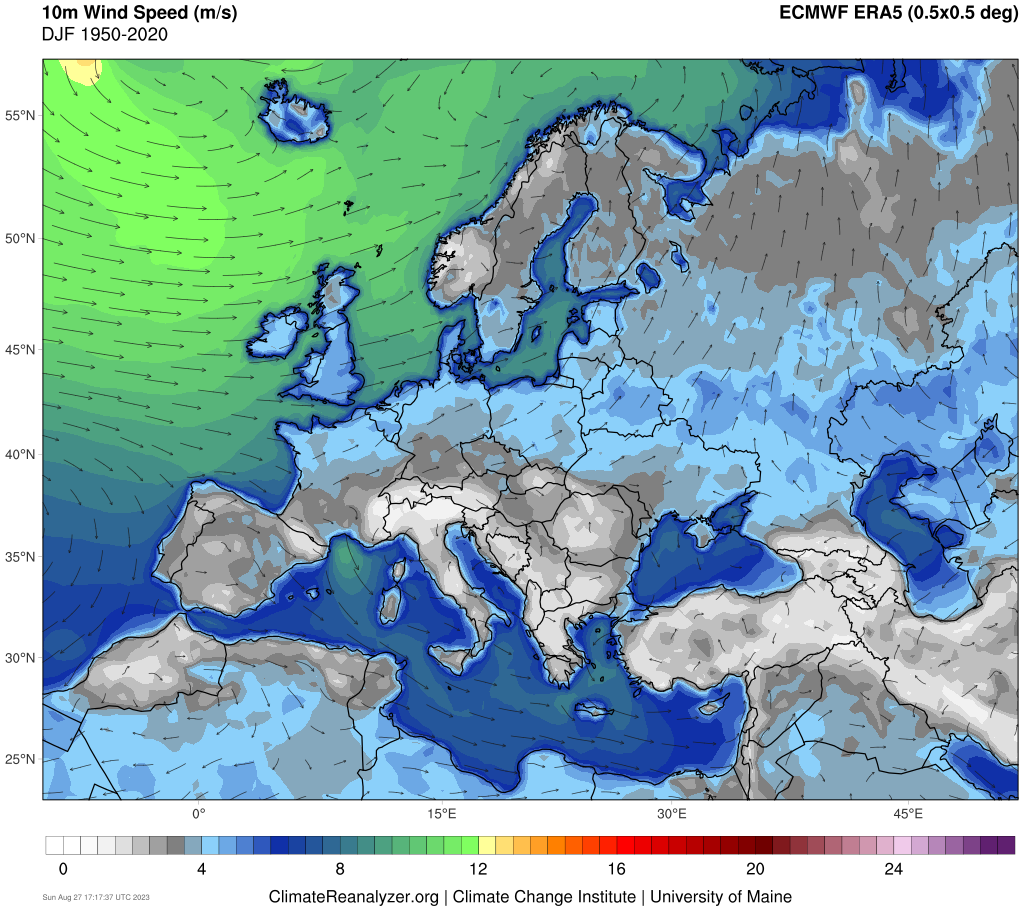
\includegraphics[width=\textwidth]{figures/era5-0p5deg_68.png}
            \caption{Sourced from \cite{ClimateReanalyzer2023}. 10m average Wind Speed in m/s for the December-January-February period over the years 1950 to 2020. Based on ECMWF ERA5 reanalysis data.}
            \label{fig:CR_10m_wind_DJF}
        \end{figure}
    
        \begin{figure}
            \centering
            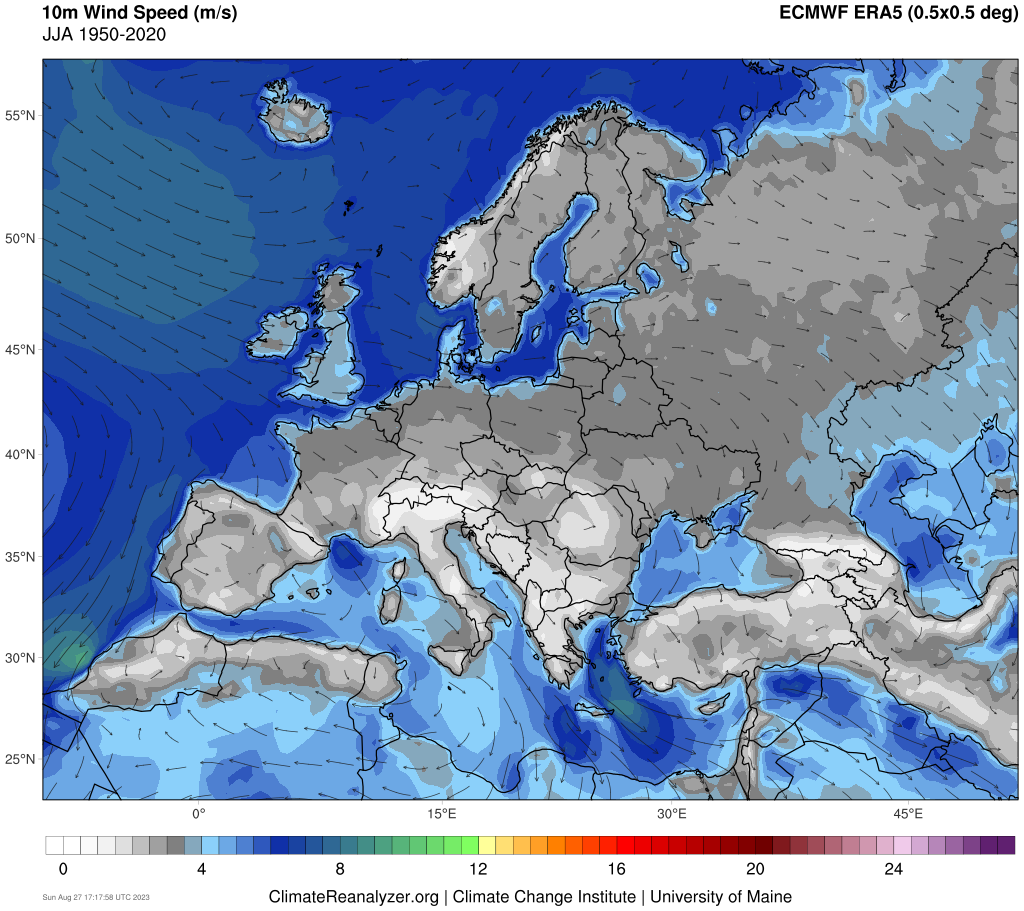
\includegraphics[width=\textwidth]{figures/era5-0p5deg_26.png}
            \caption{Sourced from \cite{ClimateReanalyzer2023}. 10m average Wind Speed in m/s for the June-July-August period over the years 1950 to 2020. Based on ECMWF ERA5 reanalysis data.}
            \label{fig:CR_10m_wind_JJA}
        \end{figure}
    
        \cite{https://doi.org/10.1002/joc.1982} and \cite{https://doi.org/10.1002/2014GL059647} observe, based on windstorm data between 1950 and 2010, that in addition to their findings aligning with those of \citeauthor{TheEffectsofNorthAtlanticSSTandSeaIceAnomaliesontheWinterCirculationinCCM3PartIMainFeaturesandStormTrackCharacteristicsoftheResponse} and \citeauthor{Hurrell2003}, windstorms are most likely to develop during moderately positive NAO phases. 
    
        In 2009, \cite{Pinto2009} published a significant statistical analysis of extreme cyclones and their relation to the NAO, as well as the variables that dominate their intesification: latent energy, upper-air baroclinicity, horizontal divergence, and jet stream strength. They explain the higher intensity of positive NAO cyclones to be due to the larger area with conditions that promote growth. \cite{HURRELL200928} similarly identify the NAO as important to the development and intensity of windstorms through its effect on the heat content of the Atlantic ocean.
    
        Using hindcasts from the 1$^{st}$ November, \cite{Renggli2011} finds a significant predictive skill for the frequency of December to February windstorms in the 1980–2001 period. Predictive skill in the 1980–2001 period is measured to be higher than that for the 1960–2001 period. Additionally, the level of skill turns out to be related to the frequency of storms in a given winter. Generally, winters with high storm frequency are better predicted than winters with medium storm frequency. Looking at their findings today, the author believes that this tendency might be due to the signal-to-noise ratio in models. Winters with high storm frequency will most likely have more ensemble members forecasting a windstorm in their simulation. As such the SNR will be higher as compared to low-windstorm frequency winters, where only few members will predict a windstorm and the forecast might be drowned out in the ensemble average.
    
        \cite{Scaifehttps://doi.org/10.1002/2014GL059637} reports on advances in modelling that allow the NAO to be predicted months in advance, this skill extending to winter storminess and wind speed. Furthermore, winter extremes are shown to be predictable, which allows for the forecasting of windstorms. \citeauthor{Scaifehttps://doi.org/10.1002/2014GL059637} use the Met Office Global Seasonal Forecast System 5 (GloSea5). They report that due to an anomalously low signal-to-noise ratio, a paradox emerging in climate models described in detail by \cite{Scaife2018}, large ensembles are needed to achieve a given level of skill. This work is expanded on by \cite{Scaife2016}, where stratospheric events such as sudden stratospheric warming (SSW) and strong polar vortex (SPV) are linked to a shift in the NAO. Similarly to \citeauthor{Scaifehttps://doi.org/10.1002/2014GL059637}, \cite{Palin2016} and \cite{Clark_2017} report on a statistically significant relationship between the NAO and hazardous weather conditions during winter in the UK, in particular of wind speed and wind power. 
    
        In 2018, for the first time, \cite{Befort2018} shows a significant ability to forecast the winter frequency of extratropical storms and high-impact windstorms associated with them, in areas prone to such events. This is an improvement over \cite{Renggli2011} as \citeauthor{Befort2018} produces a forecast, while the former report their predictive ability in hindcasts. Although the forecasts produced are statistically significant, the reported skill is still low to medium. Forecasts using the NAO as a predictor of windstorms are more successful over the British Isles and North Sea in MetOffice-GloSea5 and ECMWF-System4, but less so over central western Europe. The skill improves by combining this technique with the inclusion of an objective tracking algorithm.
    

    
    \subsection{Where we are today}

        The latest report, at the time of writing this work, is that of \cite{Degenhardt2023}. In it, two approaches to windstorm forecasting are compared by their ability to predict frequency of events during the winter season and the accumulated severity of windstorms for that season. The first method is referred to as a 'direct' method and consists of identifying and tracking storms in individual members of the seasonal hindcast ensembles in the MetOffice-GloSea5.
        The second method, named as 'indirect', is also used in \cite{Befort2018} and \cite{Scaifehttps://doi.org/10.1002/2014GL059637}. In it, storm parameters are calculated via a statistical regression, based on a combination of large-scale patterns as predictors (NAO, Scandinavian Pattern - SCA, and East-Atlantic Pattern - EA). \citeauthor{Degenhardt2023} builds a multiple linear regression model for each of the parameters they want to investigate.

        Both methods report skill similar to that of previous studies such as \cite{Befort2018} and \cite{Scaifehttps://doi.org/10.1002/2014GL059637} when the predicted parameter is the frequency of the storms. The statistical method used by \cite{Renggli2011} produces better results for winters with frequency of windstorms in the lower or upper tercile. The main difference between the direct and indirect methods is their ability to predict the severity parameter. The indirect method performs better when all predictor indices are incorporated - the NAO, SCA and EA in comparison to statistical regression methods that solely use the NAO. Despite this improvement, the indirect method is still second to the skill displayed by the direct method. In their work, \citeauthor{Degenhardt2023} report an anomalously low signal-to-noise ratio, as described in \cite{Scaife2018}, similarly to other previous studies.

        In an unpublished work, \cite{Priestley2023} explore a new statistical technique to obtain wind gusts throughout Europe using observed windstorm footprints. Through this method, high return period losses can be assessed without the complexities of a full catastrophe model.


\section{Existing SSI Methods}
    
    Having a quantitative measure of windstorm severity is important for both the private sector (research, (re)insurance) and the public sector (public safety, resource allocation). To achieve this measure, the concept of a Storm Severity Index is introduced. SSI's can be largely split into two categories: impact-based and meteorological. The former includes a measure of vulnerability, such as population or amount of infrastructure. An SSI using this measure will yield a higher index for windstorms over a town than over uninhabited areas. The latter method is concerned solely with the attributes of the storm and is a purer measure of severity. In this study, we use a meteorological method.

    \subsection{Description and Examples of Existing Methods}

        As defined in \cite{ADictionaryofWeather}, a Storm Severity Index is a measure of the severity of storms in the form of Equation \ref{eq:SSIDictionary}, where $\mathbf{V}$ is the maximum surface velocity of the wind, $\mathbf{A}$ is the largest surface area containing damaging winds and $\mathbf{D}$ is the duration of time.

        \begin{equation}
            \label{eq:SSIDictionary}
            \mathbf{V}^3 \cdot \mathbf{A} \cdot \mathbf{D}
        \end{equation}

        Of Equation \ref{eq:SSIDictionary} the one variable that remains the same in all variants of SSI is the component of the wind speed to the $3^{\text{rd}}$ power. The equation itself can be modified according to the needs of the study. An example is the SSI used by the Copernicus Extreme Windstorm Catalogue given in Equation \ref{eq:SSI_XWS}, where $\mathbf{V}_{\text{max}}$ is the maximum wind speed of the storm and $\mathbf{A}$ is the size of the storm over land for which the maximum gust exceeds 25mps. In this version of Equation \ref{eq:SSIDictionary}, the duration $\mathbf{D}$ does not appear, as this SSI is only concerned with the instant for which the storms wind is most violent. In this form of the SSI, \cite{XWS-nhess-14-2487-2014} find that the classification of windstorms best identifies those with high insurance loss.

        \begin{equation}
            \label{eq:SSI_XWS}
            \text{SSI}_{\text{XWS}} = \mathbf{V}_{\text{max}}^3 \cdot \mathbf{A}
        \end{equation}

        For another example, we can look at the SSI method used by a reinsurance company given in Equation \ref{eq:SSI_AON}. $\mathbf{V}_{\text{Filtered}}$ is given by Equation \ref{eq:SSI_AONDef} and $\mathbf{A}$ has a similar filter applied such that only the area where the winds exceed 20 meters per second is included in the sum. This method is more thorough than the XWS method as it breaks the storm into grids and considers the wind speed in each individual cell. It also uses a lower threshold and as such is more suitable when studying a broader range of storms, while the above is focused on identifying only the most severe of events.

        \begin{equation}
            \label{eq:SSI_AON}
            \text{SSI}_{\text{AON}} = \frac{\sum_{\text{Grids}}\left(\mathbf{V}_{\text{Filtered}}\right)^3 \cdot \mathbf{A}}{\mathbf{A}_{\text{Country}}}
        \end{equation}

        \begin{equation}
            \label{eq:SSI_AONDef}
            \mathbf{V}_{\text{Filtered}} = 
                \begin{cases}
                    \mathbf{V}_{\text{Wind}} - 20\left[m/s\right] & \mathbf{V}_{\text{Wind}} > 20 \\
                    0                                             & \text{otherwise} \\
                \end{cases}
        \end{equation}